\chapter{Funciones Hash}
En este capítulo voy a describir que son las funciones hash, como construirlas usando la construcción \emph{Merkle-Damgård} y por último explicaré las funciones hash más utilizadas en las aplicaciones de mensajería en la actualidad.
\section{¿Que son las funciones hash?}
Una función resumen o función hash es una función que se puede calcular mediante un algoritmo en el cual se transforma un conjunto arbitrario de datos en una nueva serie de caracteres con una longitud fija independiente del tamaño de los datos de entrada.
Estas funciones son muy utilizadas en criptografía ya que como hemos visto, en el caso de RSA el tamaño del bloque puede suponer un problema debido a que aumenta considerablemente el tiempo de ejecución.
Para ello se utilizan funciones hash, ya que mediante el uso de estas, se consigue reducir el tamaño del mensaje sin perder información.\\ La información para esta sección la he obtenido \cite{aepd}.\\

Las propiedades esperadas de una función hash son:
\begin{itemize}
	\item Se tiene que poder utilizar en contenido digital de cualquier tamaño y formato.
	\item Independientemente del tamaño de la entrada y del tipo, se produce una salida numérica de tamaño fijo.
	\item Para el mismo conjunto de datos de entrada, el resultado siempre es el mismo.
	\item Reconstruir el mensaje original a partir del generado tiene que ser muy complejo, idealmente imposible.
	\item Una variación mínima del mensaje original tiene que producir un hash totalmente distinto, esta propiedad se denomina \emph{difusión}.
	\item Dado un mensaje, tiene que ser muy difícil encontrar otro mensaje con la misma imagen que este \emph{colisión débil}.
	\item Tiene que ser muy costoso encontrar dos mensajes que tengan la misma imagen, esta propiedad es denominada \emph{colisión fuerte}.
	\item Dado un posible valor del espacio imagen, tiene que ser igual de probable que salga este u otro cualquiera. Es decir todos los valores tienen la misma probabilidad de salir.
\end{itemize}

Visto esto, en general, una función hash funciona de la siguiente forma:
\begin{enumerate}
	\item El mensaje de entrada se divide en bloques.
	\item Una fórmula calcula el hash, un valor con un tamaño fijo, para el primer bloque.
	\item Se calcula el hash del siguiente bloque y se suma con el hash calculado previamente.
	\item Se repite de manera análoga con el resto de bloques hasta que se recorren todos.
\end{enumerate}

Las hash que explicaré serán: \emph{SHA-0} y \emph{SHA-1} que son las funciones antecesoras de la función \emph{SHA-256} que es la que se utiliza mayoritariamente en las funciones de mensajería en la actualidad. Algunas también pueden utilizar SHA-1\\

\section{La construcción \emph{Merkle-Damgård}}
Antes de desarrollar las funciones hash mencionadas anteriormente, voy a describir la construcción \emph{Merkle-Damgård}. Este es un método para construir funciones hash que sean resistentes a colisiones a partir de funciones de compresión unidireccionales. La información para este apartado ha sido obtenida de \cite{Tiwari2017}.\\
Este método fue descubierto en 1989 por Merkle y Damgård de manera independiente. Es muy importante ya que gracias a este, se desarrollaron las funciones hash \emph{MD4,\:MD5,\:SHA-0,\:SHA-1 \text{ y }SHA-2} entre otras.\\
Una función de compresión es una función que toma una entrada de longitud fija y produce un resumen de longitud fija. Esta recibe dos entradas: una variable cadena y un bloque del mensaje.\\

\begin{figure}[htb]
	\centering
	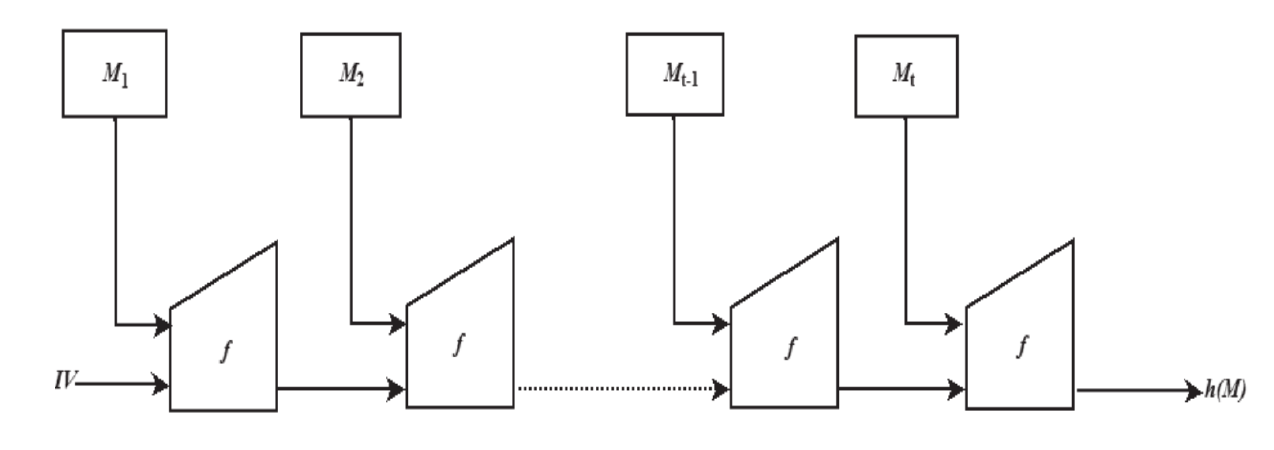
\includegraphics[scale=0.3]{imagenes/md1.png} 
	\caption{Construcción de Merkle-Damgård \cite{Tiwari2017}.}
\end{figure}
Sea $f:\{0,1\}^b\times\{0,1\}^n\rightarrow\{0,1\}^n$ una función de compresión que toma un bloque de mensajes de $b$ bits y un valor de encadenamiento de $n$ bits. Sea $h:\{0,1\}^*\rightarrow\{0,1\}^n$ una construcción \emph{MD} construida iterando la función de compresión $f$ para procesar un mensaje de longitud arbitraria. Para que esto sea posible lo que se hace es rellenar cualquier mensaje para que la longitud de este sea múltiplo de la longitud de bloque $b$ de $f$.\\
El relleno se realiza añadiendo después del último bit del último bloque del mensaje un único bit $1$ seguido del resto de bits necesarios a $0$.
Por último, para terminar de rellenar el mensaje, se añade la codificación binaria de la longitud del mensaje.\\
Una vez rellenado el mensaje, la entrada se divide en $t$ bloques, cada uno de longitud $b$. La función hash resultante puede describirse de la siguiente manera.
$$
		H_0 = IV,
$$
$$
		H_i = f(H_{i-1},M_i)\:i=1\dots t,
$$
$$
		h(M)=H_t.
$$

Este proceso se continua recursivamente, actualizando la variable cadena a partir de pasar cada bloque del mensaje por la función de compresión. La salida será la variable cadena. En \ref{mdcon} se puede ver un resumen del proceso.

\begin{figure}[htb]
	\centering
	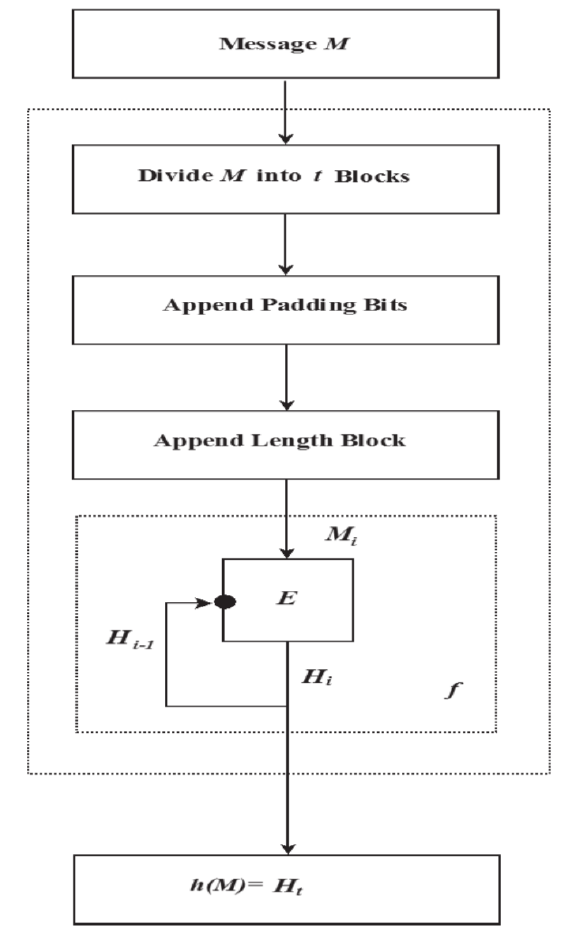
\includegraphics[scale=0.4]{imagenes/md2.png} 
	\caption{Esquema de los pasos seguidos en la construcción de Merkle-Damgård \cite{Tiwari2017}.}
	\label{mdcon}
\end{figure}

\section{SHA-0}
SHA-0 es una función hash que apareció publicada en el Federal Information Processing Standard (FIPS-180) por el NIST en 1993 \cite{Penard2008}. Está basada en \emph{MD4} y \emph{MD5}. El algoritmo transforma un mensaje de cualquier tamaño hasta $2^{64}$ bits y los transforma en un resumen de 160 bits.\\
El funcionamiento de SHA-0 es el siguiente \cite{sha0}:
\begin{enumerate}
	\item Al igual que en MD5, el mensaje se rellena con un único bit '1' seguido de 0-511 bits '0'. A continuación se añade una representación de 64 bits de la longitud del mensaje donde el número de ceros es elegido para asegurar que la longitud total del mensaje es un múltiplo de 512 bits. El mensaje se divide en bloques de 512 bits: $M_1,...,M_n$.
	\item Para la primera iteración se utiliza un buffer predefinido:
	$$
		h_0=(67452301_x, EFCDAB89_x, 98BADCFE_x, 10325476_x, C3D2E1F0_x).
	$$
	\item Cada bloque $M_j$ es pasado por la función de compresión junto con el valor actual de $h_{j-1}$, la salida es el nuevo valor de $h_j$, la operación se puede resumir en
	$$
		h_j=compresión(M_j,h_{j-1}).
	$$
	\item $h_n$ es la salida de la función hash.
\end{enumerate}
Los pasos seguidos en la función de compresión son:
\begin{enumerate}
	\item Se divide el bloque $M_j$ de 512 bits en bloques 16 bloques de 32 bits $W_0,W_1,...,W_{15}$. 
	\item Se expanden los 16 bloques de 32 bits en 80 bloques a partir de la siguiente ecuación en recurrencias:
	$$
		W_i=W_{i-3}\oplus W_{i-8}\oplus W_{i-14}\oplus W_{i-16},\; i=16,...,79.
	$$
	Esta expansión se nota como exp(.).
	\item Divide $h_{j-1}$ en 5 registros \emph{A, B, C, D} y \emph{E} como:
	$$
		h_{j-1} = (A_0, B_0, C_0, D_0, E_0).
	$$
	\item Para $i=0,...,79$ hacemos:
	$$
		A_{i+1}=(A_i\lll5)+f_i(B_i,C_i,D_i)+E_i+K_i) \mod 2^{32},
	$$
	$$
		B_{i+1}=A_i,\: C_{i+1}=(B_i\lll30),\: D_{i+1}=C_i,\: E_{i+1}=D_i.
	$$
	Donde las funciones y las constantes están definidas en la tabla \ref{tablasha0}.
	\item La salida de la función sería:
	$$
		h_n=(A_0+A_{80}, B_0+B_{80}, C_0+C_{80}, D_0+D_{80}, E_0+E_{80}).
	$$
\end{enumerate}

\begin{table}[H]
	\begin{center}
		\begin{tabular}{| l | l | l |}
				\hline
				Rondas & $f_i(B,C,D)$ & $K_i$\\ \hline
				$0\leq i\leq 19$ & $BC\vee BD$ & $5AD9EBA1_x$\\ \hline
				$20\leq i\leq 39$ & $B\oplus C\oplus D$ & $6ED9EBA1_x$\\ \hline
				$40\leq i\leq 59$ & $BC\vee BD\vee CD$ & $8F1BBCDC_x$\\ \hline
				$60\leq i\leq 79$ & $B\oplus C\oplus D$ & $CA62C1D6_x$\\ \hline
		\end{tabular}
		\caption{Funciones y constantes usadas en la función de compresión de SHA-0 \cite{sha0}.}
	\label{tablasha0}
	\end{center}
\end{table}

\section{SHA-1}
La función SHA-1 es una función hash diseñada en 1995 por la \emph{National Security Agency} (NSA) dado que que se encontraron varias colisiones y vulnerabilidades en la función SHA-0 \cite{Penard2008}.\\
Su funcionamiento es muy similar al de la función SHA-0 variando en las funciones y variables usadas en las distintas rondas de la función de compresión. En la tabla \ref{tablasha1} se pueden ver los nuevos valores utilizados.\\
\begin{table}[htb]
	\begin{center}
		\begin{tabular}{| l | l | l |}
				\hline
				Rondas & $f_i(B,C,D)$ & $K_i$\\ \hline
				$0\leq i\leq 19$ & $(B\wedge C)\oplus (\overline{B}\wedge D)$ & $5A827999_x$\\ \hline
				$20\leq i\leq 39$ & $B\oplus C\oplus D$ & $6ED6EBA1_x$\\ \hline
				$40\leq i\leq 59$ & $(B\wedge C)\oplus (B\wedge D) \oplus (C\wedge D)$ & $8FABBCDC_x$\\ \hline
				$60\leq i\leq 79$ & $B\oplus C\oplus D$ & $CA62C1D6_x$\\ \hline
		\end{tabular}
		\caption{Funciones y constantes usadas en la función de compresión de SHA-1 \cite{sha1}.}
		\label{tablasha1}
	\end{center}
\end{table}

En imagen \ref{sha01img} se puede observar un esquema del proceso para obtener un el hash seguido por las funciones  SHA-0 y SHA-1 donde \textbf{F} será la función de compresión.
\begin{figure}[htb]
	\centering
	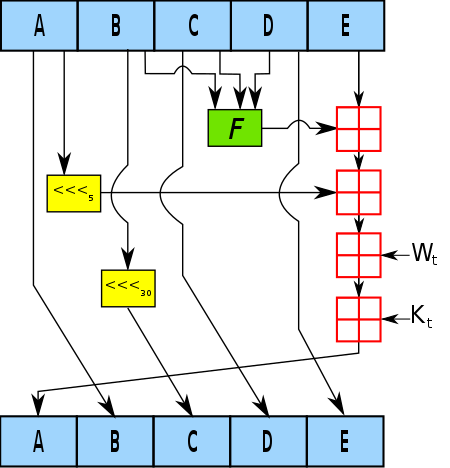
\includegraphics[scale=0.5]{imagenes/sha0-1.png} 
	\caption{Esquema de los pasos seguidos en SHA-0 y SHA-1 \cite{fotosha10}.}
	\label{sha01img}
\end{figure}

\section{SHA-256}
La función SHA-256 pertenece a la familia SHA-2 que es un conjunto de funciones hash diseñadas por la NSA en 2001 \cite{Penard2008}. Esta familia está compuesta por las funciones SHA-224, SHA-256, SHA-384 y SHA-512 donde el número del final indica el tamaño de bloque en el que se dividirá el mensaje. Nos centraremos en la función SHA-256 que como he comentado anteriormente es la que se utiliza en las aplicaciones de mensajería actualmente.\\
El funcionamiento de las función es el siguiente\cite{Function2016}:\\
\begin{enumerate}
	\item Al igual que en SHA-0 y SHA-1 se rellena el mensaje de la misma manera y se fragmenta en bloques de 512 bits: $M_1,...,M_n$.
	\item Para la primera iteración se utiliza un buffer predefinido:
	$$
		h_0=(H_1, H_2, H_3, H_4, H_5, H_6, H_7, H_8),
	$$
	donde:\\
	$H_1=6A09E776$,\\
	$H_2=BB67AE85$,\\
	$H_3=3C6EF372$,\\
	$H_4=A54FF53A$,\\
	$H_5=510E527F$,\\
	$H_6=9B05688C$,\\
	$H_7=1F83D9AB$,\\
	$H_8=5BE0CD19$.\\
	\item Cada bloque $M_j$ es pasado por la función de compresión junto con el valor actual de $h_{j-1}$, la salida es el nuevo valor de $h_j$, la operación se puede resumir en:
	$$
		h_j=compresión(M_j,h_{j-1}).
	$$
	\item $h_n$ es la salida de la función hash.
\end{enumerate}
Los pasos seguidos en la función de compresión son:
\begin{enumerate}
	\item Se divide el bloque $M_j$ de 512 bits en bloques 16 bloques de 32 bits $W_0,W_1,...,W_{15}$. 
	\item Se expanden los 16 bloques de 32 bits en 63 bloques a partir de la siguiente ecuación en recurrencias:
	$$
		W_i=\sigma_1(W_{j-2})+W_{j-7}+\sigma_0(W_{j-16}),\; i \in \{16...63\}.
	$$
	\item Divide $h_{j-1}$ en \emph{A, B, C, D, E, F, G} y \emph{H} como:
	$$
		h_{j-1} = (A_0, B_0, C_0, D_0, E_0, F_0, G_0, H_0).
	$$
	\item Para $i=0,...,63$ hacemos:
	$$
		A_{i+1}=H_i+\Sigma_1(E_i)+Ch(E_i,F_i,G_i)+K_j+W_j+\Sigma_0(A_i)+Maj(A_i,B_i,C_i),
	$$
	$$
		B_{i+1}=A_i,\: C_{i+1}=B_i,\: D_{i+1}=C_i,\: F_{i+1}=E_i\: G_{i+1}=F_i,\: H_{i+1}=G_i,
	$$
	$$
		E_{i+1}=D_i+H_i+\Sigma_1(E_i)+Ch(E_i,F_i,G_i)+K_j+W_j.
	$$
	Donde las funciones y las constantes están definidas en la tabla \ref{tablasha0}.
	\item La salida de la función es:
	$$
		h_j=(A_0+A_{63}, B_0+B_{63}, C_0+C_{63}, D_0+D_{63}, E_0+E_{63}, F_0+F_{63}, G_0+G_{63}, H_0+H_{63}).
	$$
\end{enumerate}
Donde tenemos que:
$$
	Ch(x,y,z) = (x\wedge y)\oplus (\overline{x}\wedge z),
$$
$$
	Maj(x,y,z) = (x\wedge y)\oplus (x\wedge z)\oplus (y\wedge z),
$$
$$
	\Sigma_0(x) = (x\ggg2)\oplus (x\ggg13)\oplus (x\ggg22),
$$
$$
	\Sigma_1(x) = (x\ggg6)\oplus (x\ggg11)\oplus (x\ggg25),
$$
$$
	\sigma_0(x) = (x\ggg7)\oplus (x\ggg18)\oplus (x\lll3),
$$
$$
	\sigma_1(x) = (x\ggg17)\oplus (x\ggg19)\oplus (x\lll10).
$$

En la imagen \ref{sha256img} podemos ver un esquema de los pasos seguidos en las funciones SHA-2.\\
\begin{figure}[htb]
	\centering
	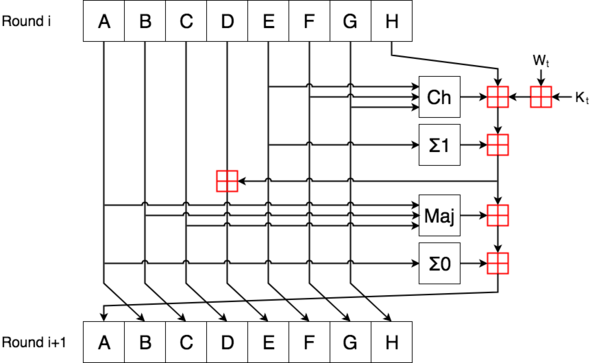
\includegraphics[scale=0.5]{imagenes/sha2.png} 
	\caption{Esquema de los pasos seguidos en las funciones de la familia SHA-2 \cite{sha2wikipedia}.}
	\label{sha256img}
\end{figure}
\newpage
Con este capítulo concluye la parte de descripción de criptosistemas y herramientas utilizadas por las aplicaciones de mensajería. En el siguiente capítulo voy a describir como utilizan estas herramientas las aplicaciones de mensajería más populares para garantizar la seguridad y la privacidad de sus usuarios.
